\documentclass[11pt]{article}
\usepackage{fullpage,amsmath,mathtools, algorithm2e, forest}
\usepackage[mathletters]{ucs}
\usepackage{hyperref}
\usepackage[utf8x]{inputenc}
\usepackage{graphicx}
\usepackage{listings}
\usepackage{courier}

\lstset{basicstyle=\footnotesize\ttfamily,breaklines=true}
\lstset{frame=single}

\graphicspath{ {./images/} }
\title{COMP4107 - Assignment 4}
\author{Student Name: Yunkai Wang\\
\text{Student Number: 100968473}\\\\
Student Name: Jules Kuehn\\
\text{Student Number: 100661464}}
\date{Fall 2018}
\begin{document}
\maketitle

\begin{enumerate}
\item Modification of the dataset loaded.\\
We modified the files so that they are all loading the CIFAR-10 datasets.
\item Changing the number of convolutional layers and sizes of max pooling layers. You must investigate 5 different model scenarios.\\
\item Provide a PDF image of your computational graph. This must be captured from TensorBoard.\\
We modified q1-original-cnn-model\_tensorboard.py file, so that when the model is created, it's separated into several layers, so that the result computational graph looks nicer. When the session runs, the graph is captured by the tensorboard. Here is how the model looks like(directly downloaded from tensorboard):
\begin{figure}[h!]
    \centering
     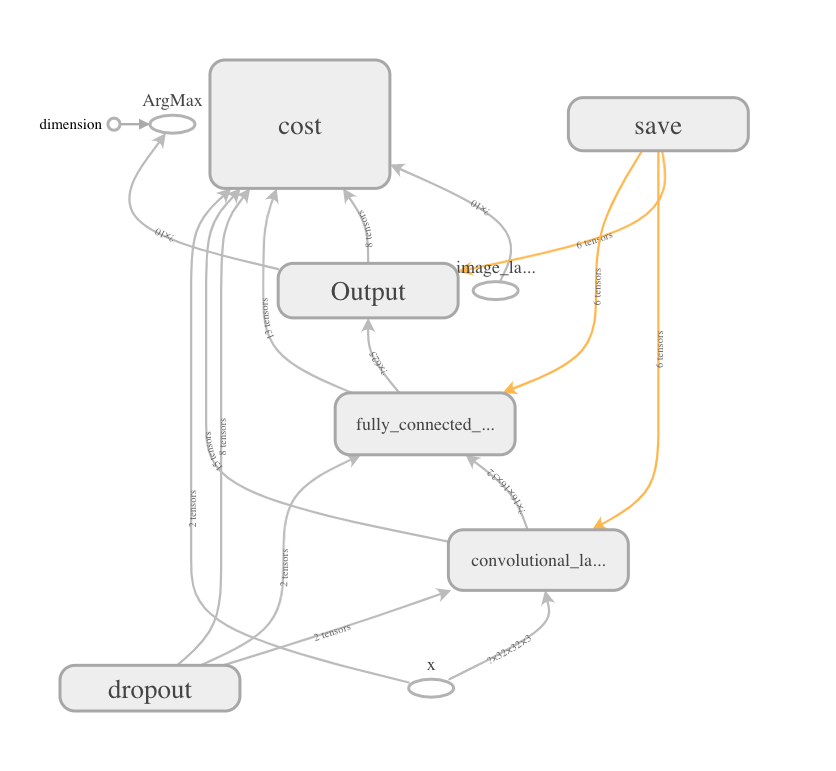
\includegraphics[width=0.5\textwidth]{images/computational_graph}
        \caption{Computational graph of the original CNN}
\end{figure}
Notice that since we group the variables by layers, so they are hidden inside those layers, but we include the generated event file, which can be used to launch the tensorboard($tensorboard --logdir=./tensorboard/original\_cnn/$), and then the graph can be expanded there. We only did add the code to one of the model just because adding the extension for all other models is simply the same thing, and the prof said that it's sufficient to include just one graph.
\item Provide a capability to view weight histograms using TensorBoard. You must be able to checkpoint your model during training. See tutorial for details.\\
Again, we made the change only in the q1-original-cnn-model\_tensorboard.py file. We saved our session after each epoch, which can be reflected at the bottom of the code. We created the following histograms(Figure 2) after we have trained our model for 50 epochs.
\begin{figure}[h!]
    \centering
     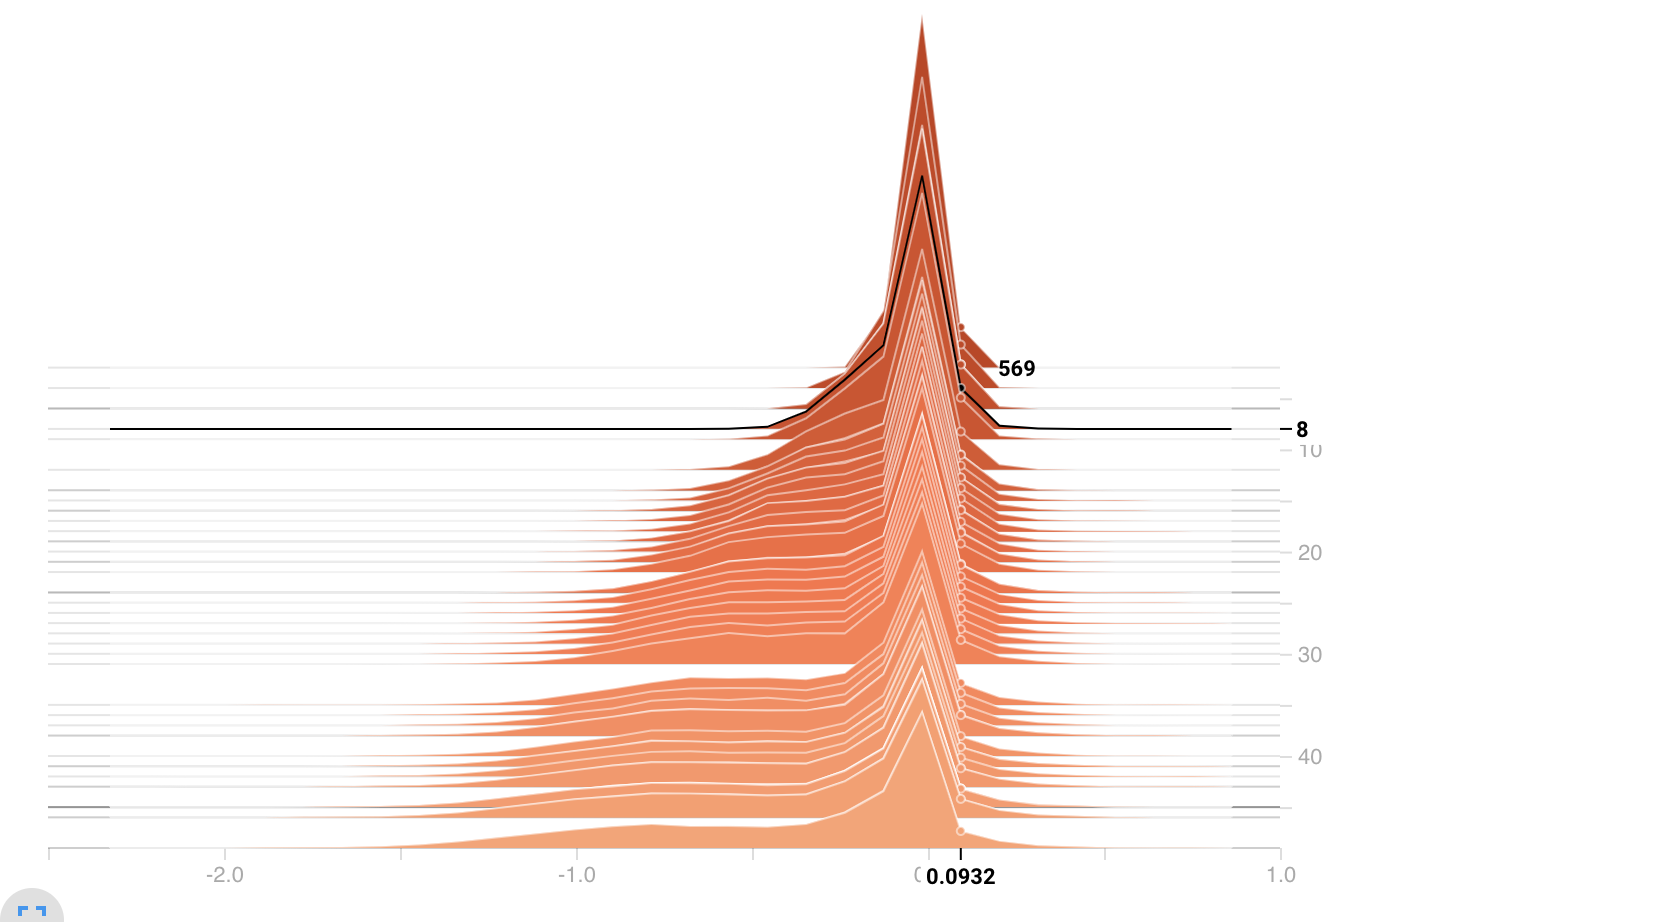
\includegraphics[width=0.5\textwidth]{images/histogram_1}
     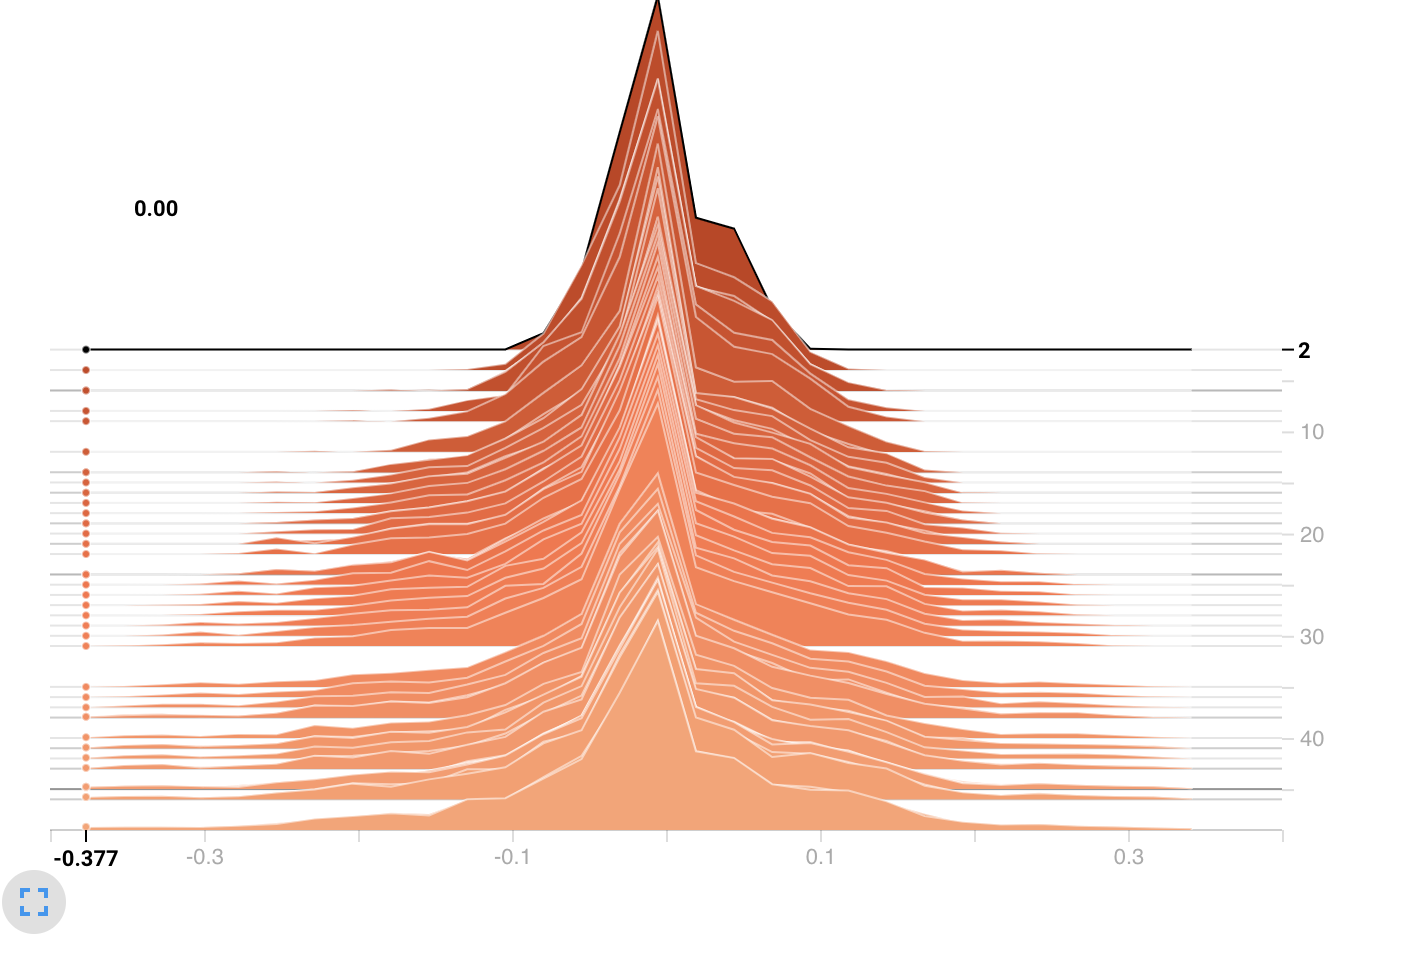
\includegraphics[width=0.5\textwidth]{images/histogram_2}
    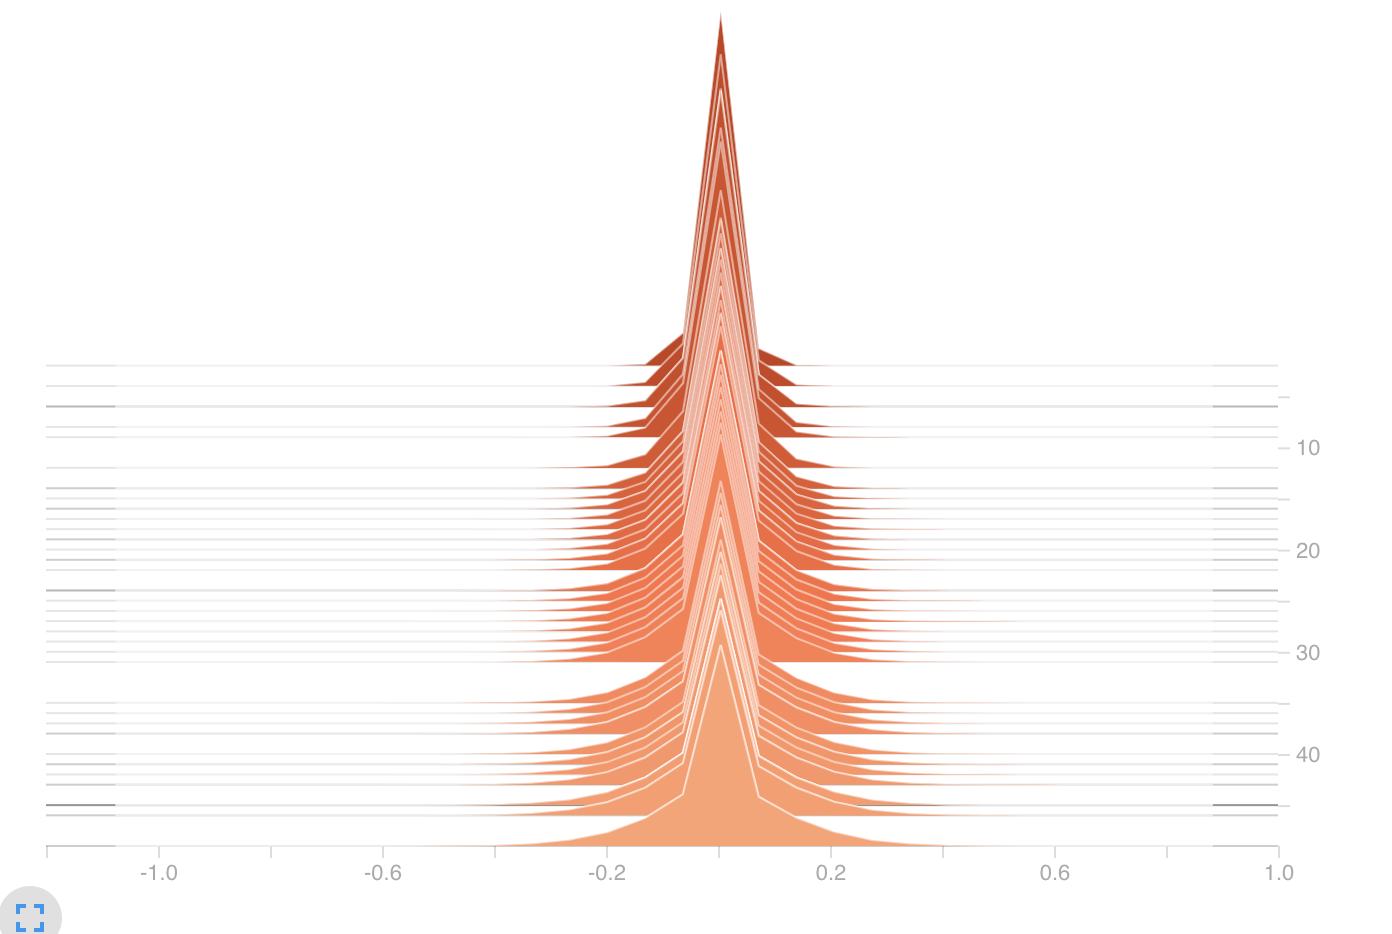
\includegraphics[width=0.5\textwidth]{images/histogram_3}
        \caption{Histograms of the weights in the model}
\end{figure}
\item Provide a chart of the accuracy of your network for 1-15 epochs for the scenarios investigated.
We trained all our 5 models for 50 epochs, and here is the accuracies combined in one graph.
\begin{figure}[h!]
    \centering
     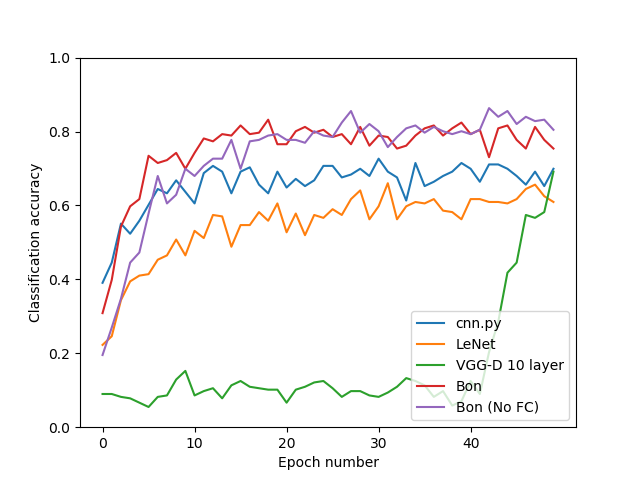
\includegraphics[width=0.75\textwidth]{images/accuracy}
        \caption{Accuracy of the CNNs}
\end{figure}
\item Provide the capability to show the top 9 patches. Examples are shown on slides 63-65 of the CNN notes.\\
The code to accomplish this task can be found in q1-bonaccorso-noFC-extra\_conv-model\_top9.py file, what we did is that we use the layer 1, and when we are given a new image, we find the top 9 neurons with the highest activation, and get the following images(Figure 4):
\begin{figure}[h!]
    \centering
     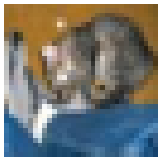
\includegraphics[width=0.25\textwidth]{images/0_input_image}
     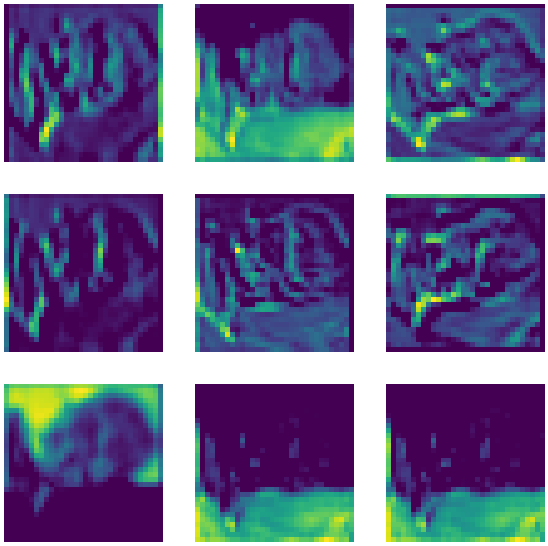
\includegraphics[width=0.25\textwidth]{images/0_top_layers}\\
     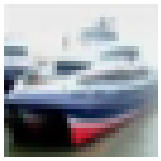
\includegraphics[width=0.25\textwidth]{images/1_input_image}
     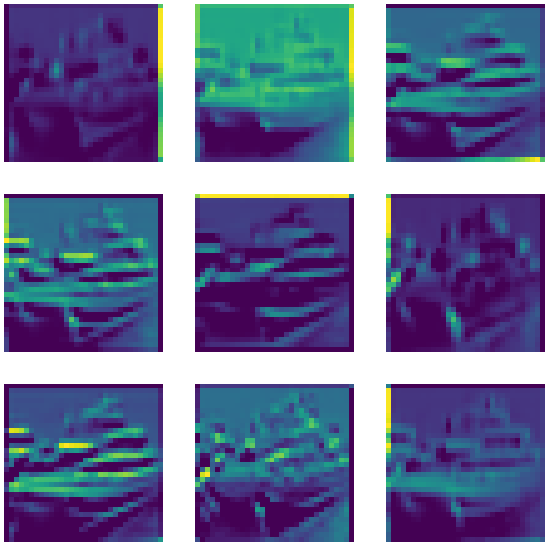
\includegraphics[width=0.25\textwidth]{images/1_top_layers}\\
     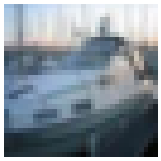
\includegraphics[width=0.25\textwidth]{images/2_input_image}
     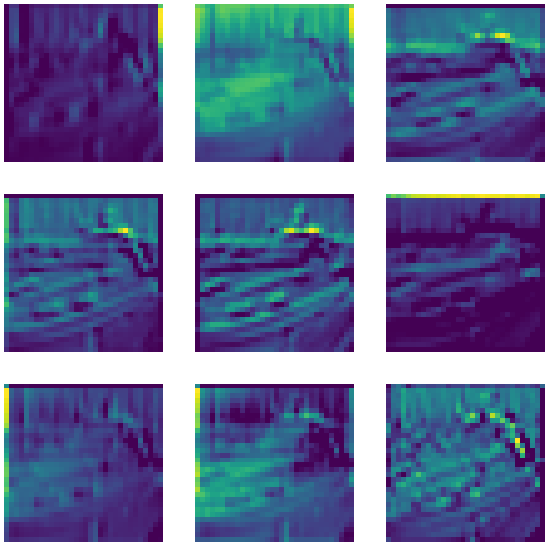
\includegraphics[width=0.25\textwidth]{images/2_top_layers}
        \caption{Top 9 patches of the given image}
\end{figure}

\end{enumerate}

\end{document}